Consider a closed loop system in the standard negative unity feedback configuration shown below
\begin{center}
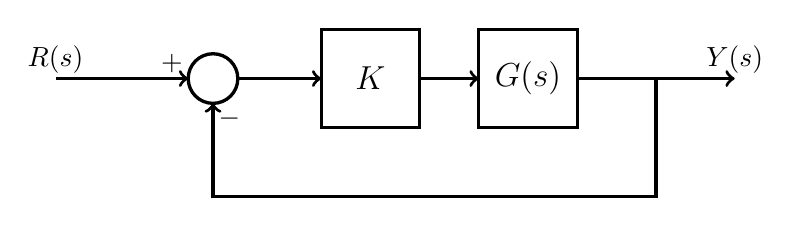
\begin{tikzpicture}[scale=1,inner sep=0pt,outer sep=0pt,very thick,
sysblock/.style={draw,rectangle,inner sep=2pt,minimum width=1.25cm,minimum height=1.25cm,very thick}]
\draw (2,0) node[draw,circle] (sum1) {$\rule{0pt}{18pt}$};
\draw (4,0) node[sysblock] (Kp) {\large $K$};
\draw (6,0) node[sysblock] (G) {\large $G(s)$};
\draw[->] (0,0) node[above=2pt] {$R(s)$} -- (sum1.180) node[above left=2pt] {$+$};
\draw[->] (sum1.0) --  (Kp);
\draw[->] (Kp) -- (G.180);
\draw[->] (G.0) -- ++(2,0) node[above=2pt] {$Y(s)$};
\draw[->] (G.0) ++(1,0) -- ++(0,-1.5) -| (sum1.-90) node[below right=2pt] {$-$};
\end{tikzpicture}
\end{center}
The pole zero map of the transfer function $G(s)$ is as follows:
\begin{center}
\includegraphics[width=3.5in]{\mainfolder/LectureNotes/\lecturefolder/HomeworkProblems/Problem05/polezeromap}
\end{center}
\begin{enumerate}[(a)]
\item Sketch the root locus of closed loop poles as $K$ goes from $0$ to $\infty$. Include arrows designating the direction the roots travel along the loci as $K$ increases. 
\item  Based on your sketch, is it possible to choose a value of $K$ such that the closed loop system is unstable?
\end{enumerate}
